\documentclass[10pt]{article}
\usepackage[english]{babel}

\usepackage{amssymb,amsmath,amstext,dsfont,amsxtra}
 \usepackage{amsthm}
\usepackage{graphicx}
\usepackage{algorithm}
\usepackage{algorithmic}
% \usepackage{subfigure}
\usepackage{appendix}
\usepackage{booktabs}

\usepackage{color}
\usepackage{microtype}

\usepackage{comment}

\usepackage{subfigure}
\usepackage{sidecap}

\usepackage{enumitem}
\usepackage{mathtools}

\usepackage[usenames,dvipsnames]{xcolor}

\usepackage{url}

% = = = = = = = = = = = = = = = = = = = = %
% = = = = =  CUSTOM COMMANDS  = = = = = %
% = = = = = = = = = = = = = = = = = = = = %

\newcommand{\R}{\mathds{R}}
\newcommand{\N}{\mathds{N}}

\newcommand{\A}{\mathcal{A}}
\newcommand{\D}{\mathcal{D}}
\renewcommand{\H}{\mathcal{H}}
\newcommand{\M}{\mathcal{M}}
\newcommand{\X}{\mathcal{X}}

% Sans-serifed

\newcommand{\K}{\mathsf{K}}
\renewcommand{\P}{\mathsf{P}}

% Greek

\newcommand{\eps}{\varepsilon}

% Bold

\renewcommand{\k}{\mathbf{k}}
\newcommand{\p}{\mathbf{p}}
\renewcommand{\r}{\mathbf{r}}
\newcommand{\x}{\mathbf{x}}
\newcommand{\eye}{\mathbf{I}}
\newcommand{\one}{\mathbf{1}}

\newcommand{\Q}{\mathbf{Q}}
\newcommand{\T}{\mathbf{T}}
\newcommand{\V}{\mathbf{V}}

\newcommand{\btheta}{\boldsymbol\theta}
\newcommand{\bmu}{\boldsymbol\mu}
\newcommand{\balpha}{\boldsymbol\alpha}

% Probability

\newcommand{\EE}[2][]{\mathbb{E}_{#1}\left[#2\right]}
\newcommand{\PP}[2][]{\mathbb{P\!}_{#1}\left[#2\right]}
\newcommand{\PPe}[2][]{\mathbb{P}^\mathbb{E}_{#1}\left[#2\right]}
\newcommand{\PPlb}[2][]{\mathbb{P}^\text{lb}_{#1}\left[#2\right]}
\newcommand{\PPub}[2][]{\mathbb{P}^\text{ub}_{#1}\left[#2\right]}
\newcommand{\PPexact}{\mathbb{P}^\text{exact}}

% Operations

\DeclareMathOperator*{\argmax}{\rm argmax}
\DeclareMathOperator*{\argmin}{\rm argmin}

% Distributions

\newcommand{\Uni}{\mathsf{Uni}}
\newcommand{\Multi}{\mathsf{Multi}}
\newcommand{\Dir}{\mathsf{Dir}}
\newcommand{\Beta}{\mathsf{Beta}}
\newcommand{\Bin}{\mathsf{Bin}}

% Other

% \newcommand{\citet}[1]{\citeauthor{#1} (\citeyear{#1})}

\providecommand{\set}[1]{\left\{#1\right\}}
\providecommand{\abs}[1]{\left\lvert#1\right\rvert}
\providecommand{\norm}[1]{\left\lVert#1\right\rVert}
\providecommand{\dprod}[1]{\left\langle#1\right\rangle}

\newcommand{\MDP}[1][r]{(\X,\A,\P,#1,\gamma)}

\newcommand{\eg}{\textit{e.g.,~}}
\newcommand{\ie}{\textit{i.e.,~}}

% \newtheorem{definition}{Definition}
% \newtheorem{theorem}{Theorem}
% \newtheorem{corollary}{Corollary}

%\newcommand{\todo}[1]{\vspace{5 mm}\par \noindent
%\framebox{\begin{minipage}[c]{0.46 \textwidth}
%\begin{center} {\color{red}\textbf{TODO:} #1} \end{center}\end{minipage}}\vspace{5 mm}\par}

\usepackage{todonotes}
%\newcommand{\todo}[1]{{\color{red} \bf TODO: \textup{ *** #1 *** }}}

\newcommand{\idea}[1]{\todo[inline,color=cyan]{#1}}
\newcommand{\todoMatthijs}[1]{\todo[inline,color=green]{#1}}
\newcommand{\todofmelo}[1]{\todo[inline,color=gray]{#1}}


%\newcommand{\citet}[1]{\citeauthor{#1} \shortcite{#1}}

\newcommand{\expected}{\mathbb{E}}

\makeatletter
\renewcommand{\maketag@@@}[1]{\hbox{\m@th\normalsize\normalfont#1}}%
\makeatother

\newcommand{\underblue}[1]{\color{SkyBlue}{\underbracket[0.5pt][2pt]{\color{black}{#1}}}\color{black}}
\newcommand{\overblue}[1]{\color{SkyBlue}{\overbracket[0.5pt][2pt]{\color{black}{#1}}}\color{black}}


% \pdfinfo{
% /Title (ICAPS Submission \#112)
% /Subject (Automated Planning and Scheduling)
% /Author (Anonymous)}

\graphicspath{{./images/}}







%\usepackage{times}
%\usepackage{graphics}

\title{Approximate Inference in factored decision models: Insights into bounding the quality of approximate POMDP planning}
%\subtitle{idea draft}
\author{Stefan J. Witwicki and Francisco S. Melo}

\begin{document}

\newtheorem{definition}{Definition}
\newtheorem{theorem}{Theorem}

\maketitle

\section{Overview}

This document is organized by problem context.  We begin by exploring approximate inference in the original context of event prediction (as it was treated in our ARMS Workshop paper).  Then we turn to the more general case of planning for arbitrary POMDPs.

\section{Approximate Inference in Event Prediction}

\subsection{Event Model as a factored POMDP}

Figure \ref{Fig:D-separation} describes the decision model whose state has been factored, $X=\langle X_{E}, X_{U}, X_{I}\rangle$,  into \emph{latent} external variables $X_{E}$, \emph{observable} \emph{uncontrollable} event variables $X_{U}$ (which can actually be affected indirectly), and observable internal variables $X_{I}$.

\begin{figure}[h]%\begin{SCfigure}[3][!tb]
\centering
  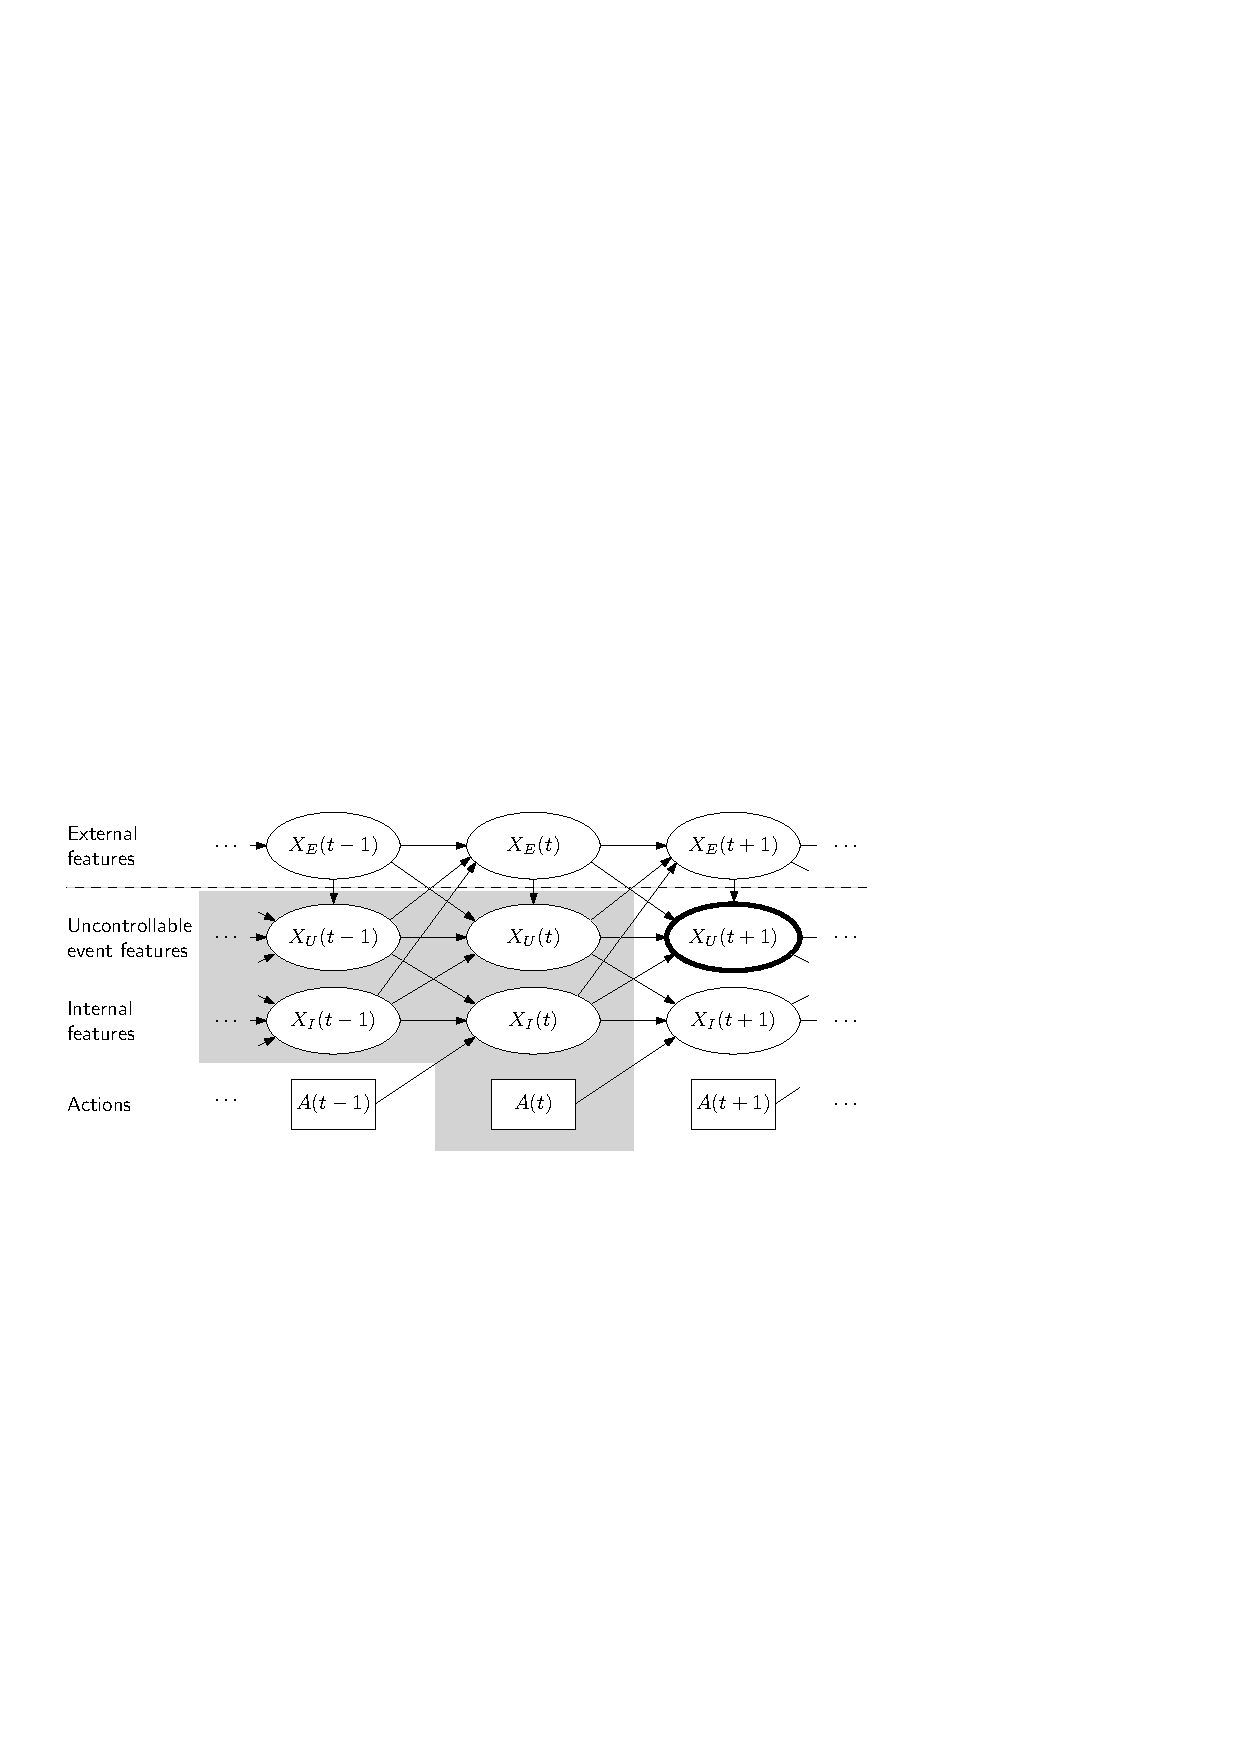
\includegraphics[width=\columnwidth]{bayes-dsep2}
%   \caption{An illustration of the d-separation of $X_U(t\!+\!1)$ and 
% %$\left\{ X_{I}(0\ldots t\!-\!1),A(0\ldots t)\right\}$ 
% $\left\{A(0\ldots t)\right\}$ 
% by the grayed region.}
\caption{A decision model (as a DBN) with distinguished uncontrollable events.}
  \label{Fig:D-separation}
\end{figure}

\noindent As indicated by the connections in the DBN above, state transitions are subject to the following assumptions:
\begin{itemize}%[label=\quad\quad\alph*)] 
\item the uncontrollable event features and the external features are conditionally independent of the agent's action $\PP{X_{U}(t+1),X_{E}(t+1)|X(t),A(t)} = \PP{X_{U}(t+1),X_{E}(t+1)|X_{E}(t),X_{U}(t),X_{I}(t)}$
\item the internal features are conditionally independent of the external features as well as concurrent events
$\PP{X_{I}(t\!+\!1)|X(t),A(t),X_{U}(t\!+\!1)} = \PP{X_{I}(t\!+\!1)|X_{U}(t),X_{I}(t),A(t)}$,
\end{itemize}
Rewards may depend on any or all factors, though observations are assumed to be equal to the variables below the dotted line.

A key property of the above Event model is that it is reducible, via inference, to an equivalent model that omits the external factors (above the dotted line).  Essentially, predictions about events (encoded by the CPT of $X_U(t\!+\!1)$) can be made from histories of non-external features $\langle X_U(0\ldots t), X_I(0\ldots t) \rangle$.  Such history, or perhaps even a subset thereof (depending on the problem), together with the latest action $A(t)$, D-separates all other variables at stages $0\ldots t$ from all of its observations at stage $t+1$, and thereby serves as a sufficient statistic for optimal planning.  This is indicated by the grey region in Figure \ref{Fig:D-separation}.  A formal statement and proof of the reducibility of the even model as such is detailed in the appendix.

Figure \ref{Fig:reduced-model} shows the general form of the reduced event model.  Note that in the reduced model, event variable $X_U(t+1)$ depends on the entire history $\langle X_U(0\ldots t), X_I(0\ldots t) \rangle$ whereas internal variable $X_I(t+1)$ depends only on variables at the previous stage $\langle X_U(t), X_I(t), A(t) \rangle$.

\begin{figure}[h]%\begin{SCfigure}[3][!tb]
\centering
  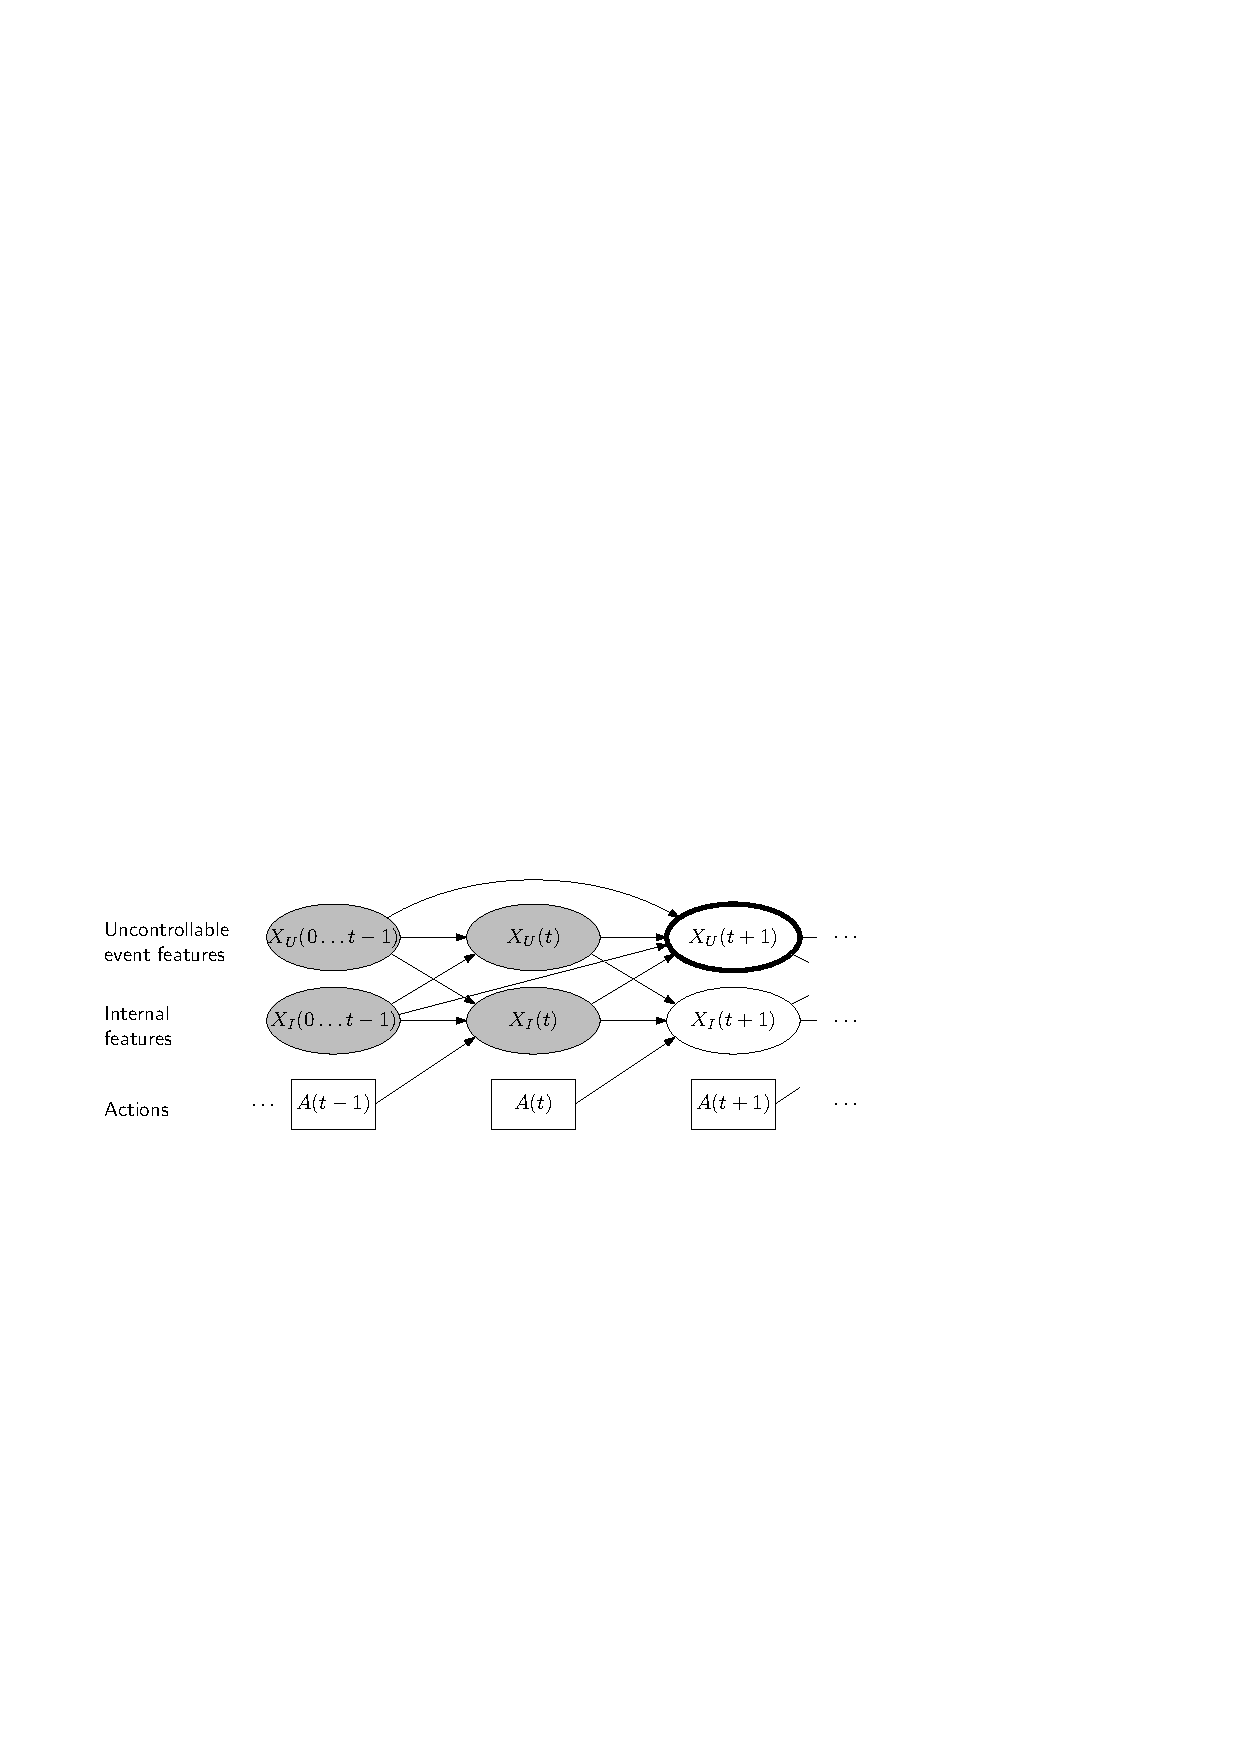
\includegraphics[width=\columnwidth]{bayes-reduced}
\caption{The general form of the reduced event model, where the greyed nodes comprise the belief state (which is augmented with history) at stage $t$.}
  \label{Fig:reduced-model}
\end{figure}

Next we describe an iterative inference algorithm for reducing the model in Figure \ref{Fig:D-separation} to that in Figure \ref{Fig:reduced-model}.

\pagebreak
\subsection{Inference Process}
\label{sec:inference-process}

Intuitively, inference can be used to eliminate external variables from the event model, one by one, starting with $X_E(0)$ and proceeding forward to $X_E(T)$ at an arbitrary (though finite) horizon $T$.  
For each stage $t$, the variable elimination consists of two steps:
\begin{enumerate}
 \item Compute the joint distribution $\boldsymbol{J}$ of $X_E(t)$ and $X_U(t)$ conditioned only on non-external history
\begin{multline}
\boldsymbol{J}(t)\equiv \PP{X_{E}(t),X_{U}(t)|X_{U}(0\ldots t\!-\!1),X_{I}(0\ldots t\!-\!1)}\\
\shoveleft
{
\quad\quad
=\sum_{X_{E}(t\!-\!1)}
\Bigg(
\PP{X_{U}(t)|X_{E}(t),X_{E}(t\!-\!1),X_{U}(t\!-\!1),X_{I}(t\!-\!1)}
}
\\
\PP{X_{E}(t)|X_{E}(t\!-\!1),X_{U}(t\!-\!1),X_{I}(t\!-\!1)}
\frac{
\boldsymbol{J}(t\!-\!1)
}{
  \sum_{X_{E}'(t\!-\!1)} \boldsymbol{J}(t\!-\!1)
}
\Bigg),
\label{eq:joint}
\end{multline}
where $\boldsymbol{J}(0) = \PP{X_{U}(0)|X_{E}(0)} \PP{X_{E}(0)}$.

\item Marginalize over the external variable $X_E(t)$, yielding the reduced CPT of $X_U(t)$ in the reduced model 
\begin{multline}
\PP{X_{U}(t)|X_{U}(0\ldots t\!-\!1),X_{I}(0\ldots t\!-\!1)} = 
\sum_{X_{E}(t)} 
\boldsymbol{J}(t)
\label{eq:cpt-after-marginalization}
\hfill
\end{multline}
\end{enumerate}
After performing these two steps, $X_E(t)$ is no longer needed in order to predict $X_U(t)$.  Nor is it needed to predict subsequent values of $X_U$ since it is only iterated over in the next iteration of inference at stage $t+1$, and not used at all in subsequent stages (evident from the fact that Equations \ref{eq:joint}-\ref{eq:cpt-after-marginalization} make no reference to $X_E(0\ldots t\!-\!2)$).  Notice that the two-step inference process only uses the joint distribution, $\boldsymbol{J}(t\!-\!1)$, computed in the previous step, and the CPTs, $\PP{X_{E}(t)|\cdots})$ and $\PP{X_{U}(t)|\cdots})$, from the original model.  The CPT for internal variables, $\PP{X_{I}(t)|\cdots})$, remains unchanged when reducing the model.
  
If the reward function $r(X(t),A(t))$ from the original model contained in its scope $X_{E}(t)$ (suggesting that rewards depend on external variable values), that too should be updated as we perform inference.  The reward function $r\prime()$ in the reduced model is simply computed from the original reward function $r()$ and the recursively-computed joint distribution $\boldsymbol{J}(t)$ from Equation \ref{eq:joint}:

{
\small
\begin{align}%
\nonumber%
\lefteqn{r\prime\!\left(X_{U}(0\ldots t),X_{I}(0\ldots t),A(t)\right)}\\
  \nonumber%
  &\qquad=\sum_{X_{E}(t)} \PP{X_{E}(t)|X_{U}(0\ldots t),X_{I}(0\ldots t)} r\!\left(X_{E}(t),X_{U}(t),X_{I}(t),A(t)\right)\\ 
  &\qquad=\sum_{X_{E}(t)}
  \left(
  \frac{
    \boldsymbol{J}(t)
  }{
    \sum_{X_{E}'(t)} \boldsymbol{J}(t)
  }
  \,r\!\left(X_{E}(t),X_{U}(t),X_{I}(t),A(t)\right)
  \right)
  \label{eq:induced-reward}
\end{align}
}

%  consists of a marginalization over $E(t)$ that transforms the probability distribution of $X_E(t+1)$ as well as that of $X_U(t+1)$.  This variable elimination operation can be broken into two steps:
% 
% {
% \small
% \begin{multline}
% \boldsymbol{J}(t)\equiv \PP{X_{E}(t),X_{U}(t)|X_{U}(0\ldots t\!-\!1),X_{I}(0\ldots t\!-\!1)}\\
% \shoveleft
% {
% \quad\quad
% =\sum_{X_{E}(t\!-\!1)}
% \Big(
% \PP{X_{U}(t)|X_{E}(t),X_{E}(t\!-\!1),X_{U}(t\!-\!1),X_{I}(t\!-\!1)}
% }
% \\
% \PP{X_{E}(t)|X_{E}(t\!-\!1),X_{U}(t\!-\!1),X_{I}(t\!-\!1)}
% \\
% \underbrace{
% \PP{X_{E}(t\!-\!1)|X_{U}(0\ldots t\!-\!1),X_{I}(0\ldots t\!-\!1)}
% }_{
% \equiv \boldsymbol{IE}(t\!-\!1)
% }
% \,\Big)
% \label{eq:joint}
% \end{multline}
% }
% {
% \small
% \begin{multline}
% \boldsymbol{M}(t)\equiv \PP{X_{U}(t)|X_{U}(0\ldots t\!-\!1),X_{I}(0\ldots t\!-\!1)} = 
% \sum_{X_{E}(t)} 
% \boldsymbol{J}(t)
% \label{eq:cpt-after-marginalization}
% \hfill
% \end{multline}
% }
% %
% {
% \small
% \begin{equation} 
% \boldsymbol{IE}(t)\equiv\PP{X_{E}(t)|X_{U}(0\ldots t),X_{I}(0\ldots t)}=
% \displaystyle\frac{
% \boldsymbol{J}(t)
% }{
% \boldsymbol{M}(t)
% }
% \hfill
% \label{eq:induced-external}
% \end{equation}
% }
% 
% 
% Inference 

\subsection{$k$-order Approximate Inference}

The variable elimination algorithm described in Section \ref{sec:inference-process} performs exact inference.   That is, although the scope (i.e., the columns and rows) of the event CPT is reduced\footnote{Note that the term ``reduction'' here is slightly misleading, suggesting a smaller CPT, though really we are replacing a dependence on external variables with a dependence on history.}   from $\PP{X_{U}(t)|X_{E}(t),X_{E}(t\!-\!1),X_{U}(t\!-\!1),X_{I}(t\!-\!1)}$ to $\PP{X_{U}(t)|X_{U}(0\ldots t\!-\!1),X_{I}(0\ldots t\!-\!1)}$, the model still yields exact probabilities of 
events which were consistent with those from the original model.

Consider now a further reduction in scope that saves storage space and computation (of inference, but more importantly of planning with the reduced model) but that \emph{does not} necessarily yield exact probabilities.  The idea is to condition the probabilities of events on a partial history of length $k$ instead of a full history: $\PP{X_{U}(t)|X_{U}(t\!-\!k\ldots t\!-\!1),X_{I}(t\!-\!k\ldots t\!-\!1)}$.  In the most extreme case, we have a zero-order approximation, inferring an approximate distribution $\PP{X_{U}(t)}$ that is independent of time $t$ and of any previous state information.

Because we are removing potentially-crucial dependencies, haphazardly cutting arrows from the DBN in Figure \ref{Fig:reduced-model}, our model will no longer serve to provide the decision-maker with exact event probabilities $\PP{X_{U}(t)|\cdots}$.  At best, we can infer expectations (i.e., marginalizing over forgotten history from stages $0\dots t\!-\!k\!-\!1$),
\begin{multline}
\small
\PPe{X_{U}(t)|X_{U}(t\!-\!k\ldots t\!-\!1),X_{I}(t\!-\!k\ldots t\!-\!1)} =\\
\mathbb{E}_{
X_{U}(0\dots t\!-\!k\!-\!1),X_{I}(0\dots t\!-\!k\!-\!1)
}\Big[ \PP{X_{U}(t)|X_{U}(0\ldots t\!-\!1),X_{I}(0\ldots t\!-\!1)} \Big],
\end{multline}
or bounds,
\begin{equation}
\small
\PPlb{X_{U}(t)|\cdots} \leq 
\PP{X_{U}(t)|X_{U}(0\ldots t\!-\!1),X_{I}(0\ldots t\!-\!1)}
\geq \PPub{X_{U}(t)|\cdots},
\end{equation}
over the possible values of entries in $\PP{X_{U}(t)|X_{U}(t\!-\!k\ldots t\!-\!1),X_{I}(t\!-\!k\ldots t\!-\!1)}$ considering all potential values of forgotten history from stages $0\dots t\!-\!k\!-\!1$.

\todo[inline]{similarly for induced rewards}

Fortunately, we can compute expectations and bounds using slight variations of the same inference process described in Section \ref{sec:inference-process}.  We present these variations in the subsections that follow.
\pagebreak
\subsubsection{Inferring expected probabilities}
% \vspace{-5mm}
\todo[inline]{This part turned out to be quite a bit more complicated than I originally envisioned (the equations below could be simplified slightly, perhaps, but not much!), and \textit{expectations} may not be so useful for us.  The \textit{bounds} computed in the next section are more important.} 
{
\small
\begin{multline}
\boldsymbol{J}^\mathbb{E}(t)\equiv \PPe{X_{E}(t),X_{U}(t)|X_{U}(t\!-\!k\ldots t\!-\!1),X_{I}(t\!-\!k\ldots t\!-\!1)}\\
\shoveleft
{
\quad\quad\,\,\,
=\sum_{X_{E}(t\!-\!1)}
\Bigg(
\PP{X_{U}(t)|X_{E}(t),X_{E}(t\!-\!1),X_{U}(t\!-\!1),X_{I}(t\!-\!1)}
}
\\
\left.
\PP{X_{E}(t)|X_{E}(t\!-\!1),X_{U}(t\!-\!1),X_{I}(t\!-\!1)}
\frac{
\sum_{\substack{X_{U}(t\!-k\!-\!1),\\X_{I}(t\!-k\!-\!1)}} \boldsymbol{J}^\mathbb{E}(t\!-\!1) \boldsymbol{M}^\mathbb{E}(t\!-k\!-\!1)
}{
  \sum_{X_{E}'(t\!-\!1)} \sum_{\substack{X_{U}(t\!-k\!-\!1),\\X_{I}(t\!-k\!-\!1)}} \boldsymbol{J}^\mathbb{E}(t\!-\!1) \boldsymbol{M}^\mathbb{E}(t\!-k\!-\!1)
}
\right),%\Bigg),
\label{eq:joint-expected}
\end{multline}
where $\boldsymbol{M}$ denotes the marginal distribution (of non-external state), in turn recursively defined, and requiring an assumption regarding action selection\footnote{In order to compute a proper expectation over event probabilities, we need to track the marginal distribution over non-external state, which is dependent on action.  As we do not have the full action history (since we want to build an event prediction model that depends on that), we need to make some simplifying assumption about how actions were chosen.  For instance, here let as assume that actions are taken from uniform-random stationary policy $\pi$.}:
\begin{multline}
\boldsymbol{M}^\mathbb{E}(t) \equiv \PP{X_{U}(t),X_{I}(t)} \\
\shoveleft{\quad\quad\quad
=
\sum_{\substack{X_{U}(t\!-\!k\ldots t\!-\!1),\\X_{I}(t\!-\!k\ldots t\!-\!1),\\A(t\!-\!1)}} 
\bigg(
\PP{X_{U}(t)|X_{U}(t\!-\!k\ldots t\!-\!1),X_{I}(t\!-\!k\ldots t\!-\!1)}
}\\
\PP{X_{I}(t)|X_{U}(t\!-\!1),X_{I}(t\!-\!1),A(t\!-\!1)}Pr(A(t\!-\!1)|X_{U}(t\!-\!1),X_{I}(t\!-\!1),\pi)
\,\boldsymbol{T}^\mathbb{E}(t-1) \bigg),
\end{multline}
where $\boldsymbol{T}$ denotes the total probability distribution (of non-external state):
\begin{multline}
\boldsymbol{T}^\mathbb{E}(t) \equiv \PP{X_{U}(t\!-\!k\!+\!1\ldots t),X_{I}(t\!-\!k\!+\!1\ldots t)}\\
\shoveleft{\quad\quad\quad
=
\sum_{\substack{X_{U}(t\!-\!k\!-\!2),\\X_{I}(t\!-\!k\!-\!2),\\A(t\!-\!1)}} 
\bigg(
\PP{X_{U}(t)|X_{U}(t\!-\!k\ldots t\!-\!1),X_{I}(t\!-\!k\ldots t\!-\!1)}
}\\
\PP{X_{I}(t)|X_{U}(t\!-\!1),X_{I}(t\!-\!1),A(t\!-\!1)}Pr(A(t\!-\!1)|X_{U}(t\!-\!1),X_{I}(t\!-\!1),\pi)
\boldsymbol{M}^\mathbb{E}(t-k-2) \bigg).
\end{multline}

% where $\boldsymbol{J}(0) = \PP{X_{U}(0)|X_{E}(0)} \PP{X_{E}(0)}$.
\begin{multline}
\PPe{X_{U}(t)|X_{U}(t\!-\!k\ldots t\!-\!1),X_{I}(t\!-\!k\ldots t\!-\!1)} = 
\sum_{X_{E}(t)} 
\boldsymbol{J}^\mathbb{E}(t)
\label{eq:cpt-after-marginalization-expected}
\hfill
\end{multline}
}

\subsubsection{Inferring probability bounds}
\label{sec:inferring-bounds}

The idea is that, for each stage $t$, we can compute two versions of the joint probability term $\boldsymbol{J}(t)$ from our original inference algorithm: a lower bound $\boldsymbol{J}^\text{lb}(t,k)$ and an upper bound $\boldsymbol{J}^\text{ub}(t,k)$, both of which are conditioned on a $k$-length history instead of the full history.\\

\noindent For stages $t\leq k$, we perform the inference algorithm exactly as specified in Section \ref{sec:inference-process}, since the $k$-length history \emph{is} a complete history:

\begin{equation}
 \boldsymbol{J}^\text{lb}(t\leq k,k)=\boldsymbol{J}^\text{ub}(t\leq k,k)=\boldsymbol{J}(t\leq k)
 \label{eq:approximate-inference-base-stages}
\end{equation}

\noindent For stages $t>k$:
\begin{multline}
\small
\boldsymbol{J}^\text{lb}(t,k)\equiv \PPlb{X_{E}(t),X_{U}(t)|X_{U}(t\!-\!k\ldots t\!-\!1),X_{I}(t\!-\!k\ldots t\!-\!1)}\\
\shoveleft
{
\quad\quad\,\,\,
=\sum_{X_{E}(t\!-\!1)}
\Bigg(
\PP{X_{U}(t)|X_{E}(t),X_{E}(t\!-\!1),X_{U}(t\!-\!1),X_{I}(t\!-\!1)}
}
\\
\left.
\PP{X_{E}(t)|X_{E}(t\!-\!1),X_{U}(t\!-\!1),X_{I}(t\!-\!1)}
\frac{
\displaystyle\min_{\substack{X_{U}(t\!-k\!-\!1),\\X_{I}(t\!-k\!-\!1)}} \boldsymbol{J}^\text{lb}(t\!-\!1,k)
}{
  \displaystyle\sum_{X_{E}'(t\!-\!1)} 
  \displaystyle\max_{\substack{X_{U}(t\!-k\!-\!1),\\X_{I}(t\!-k\!-\!1)}} \boldsymbol{J}^\text{ub}(t\!-\!1,k) 
}
\right)%\Bigg),
\label{eq:joint-min}
\end{multline}

\begin{multline}
\small
\boldsymbol{J}^\text{ub}(t,k)\equiv \PPub{X_{E}(t),X_{U}(t)|X_{U}(t\!-\!k\ldots t\!-\!1),X_{I}(t\!-\!k\ldots t\!-\!1)}\\
\shoveleft
{
\quad\quad\,\,\,
=\sum_{X_{E}(t\!-\!1)}
\Bigg(
\PP{X_{U}(t)|X_{E}(t),X_{E}(t\!-\!1),X_{U}(t\!-\!1),X_{I}(t\!-\!1)}
}
\\
\left.
\PP{X_{E}(t)|X_{E}(t\!-\!1),X_{U}(t\!-\!1),X_{I}(t\!-\!1)}
\frac{
\displaystyle\max_{\substack{X_{U}(t\!-k\!-\!1),\\X_{I}(t\!-k\!-\!1)}} \boldsymbol{J}^\text{ub}(t\!-\!1,k)
}{
  \displaystyle\sum_{X_{E}'(t\!-\!1)} 
  \displaystyle\min_{\substack{X_{U}(t\!-k\!-\!1),\\X_{I}(t\!-k\!-\!1)}} \boldsymbol{J}^\text{lb}(t\!-\!1,k) 
}
\right)%\Bigg),
\label{eq:joint-max}
\end{multline}

\noindent For all stages, inferring bounds on the event probabilities is, just like in the original inference algorithm, a simple marginalization.
\begin{multline}
\PPlb{X_{U}(t)|X_{U}(t\!-\!k\ldots t\!-\!1),X_{I}(t\!-\!k\ldots t\!-\!1)} = 
\sum_{X_{E}(t)} 
\boldsymbol{J}^\text{lb}(t,k)
\label{eq:cpt-after-marginalization-min}
\hfill
\end{multline}

\begin{multline}
\PPub{X_{U}(t)|X_{U}(t\!-\!k\ldots t\!-\!1),X_{I}(t\!-\!k\ldots t\!-\!1)} = 
\sum_{X_{E}(t)} 
\boldsymbol{J}^\text{ub}(t,k)
\label{eq:cpt-after-marginalization-max}
\hfill
\end{multline}

\todo[inline]{similarly for induced rewards}

\subsubsection{Correctness of bounds}



\begin{theorem}
\label{thm:bounds-on-joint-probability}
For the joint probability terms computed through inference in Sections \ref{sec:inference-process} and \ref{sec:inferring-bounds},
the following inequalities hold:
\begin{equation*}
\forall t\geq0, \forall k\geq0,\quad \boldsymbol{J}^\text{lb}(t,k) \leq \boldsymbol{J}(t) \leq \boldsymbol{J}^\text{ub}(t,k) 
\end{equation*}
wherein $\boldsymbol{J}^\text{lb}(t,k)$, $\boldsymbol{J}^\text{ub}(t,k)$, and $\boldsymbol{J}(t)$ refer to conditional probability tables:
\begin{align*}
&\boldsymbol{J}^\text{lb}(t,k)\equiv \PPlb{X_{E}(t),X_{U}(t)|X_{U}(t\!-\!k\ldots t\!-\!1),X_{I}(t\!-\!k\ldots t\!-\!1)};\\
&\boldsymbol{J}^\text{ub}(t,k)\equiv \PPub{X_{E}(t),X_{U}(t)|X_{U}(t\!-\!k\ldots t\!-\!1),X_{I}(t\!-\!k\ldots t\!-\!1)};\\
&\boldsymbol{J}(t)\equiv \PP{X_{E}(t),X_{U}(t)|X_{U}(0\ldots t\!-\!1),X_{I}(0\ldots t\!-\!1)},
\end{align*}
and where the $\leq$ operator signifies that, for the two tables being compared, and for any setting of variable values $\left(\forall X_{E}(t),X_{U}(0\ldots t),X_{I}(0\ldots t\!-\!1)\right)$, the (scalar) probability value of the corresponding element in the first table is less than that of the corresponding element in the second table.
\end{theorem}

\begin{proof}
% [Proof (by Induction).\\] 
Let $P_1(t)$ and $P_2(t)$ denote the inequalities to be proven.
\begin{eqnarray*}
P_1(t): \forall k\geq 0, \boldsymbol{J}(t) \geq \boldsymbol{J}^\text{lb}(t,k) \\
P_2(t): \forall k\geq 0, \boldsymbol{J}(t) \leq \boldsymbol{J}^\text{ub}(t,k)
\end{eqnarray*}

\noindent To be more concise, let us also employ the following notational shorthands.
\begin{itemize}
 \item $\textbf{CPT}\!\left[X_{U}(t)\right] \equiv \PP{X_{U}(t)|X_{E}(t),X_{E}(t\!-\!1),X_{U}(t\!-\!1),X_{I}(t\!-\!1)}$
 \item $\textbf{CPT}\!\left[X_{E}(t)\right] \equiv \PP{X_{E}(t)|X_{E}(t\!-\!1),X_{U}(t\!-\!1),X_{I}(t\!-\!1)}W$
\end{itemize}


\noindent We can prove both $P_1(t)$ and $P_2(t)$ by induction on $t$.\\

\noindent \underline{Base case} ($t\leq k$): By definition (Equation \ref{eq:approximate-inference-base-stages}), when $t\leq k$, 
$\boldsymbol{J}^\text{lb}(t,k)=\boldsymbol{J}^\text{ub}(t,k)=\boldsymbol{J}(t)$.
Thus, $\forall t \leq k$, $P_1(t)$ and $P_2(t)$ hold.\\
% Thus, by Eqns. \{\ref{eq:cpt-after-marginalization}, \ref{eq:cpt-after-marginalization-min}--\ref{eq:cpt-after-marginalization-max}\}, $\PPlb{X_{U}(t)|\cdots} = \PPub{X_{U}(t)|\cdots} = \PP{X_{U}(t)|\cdots}$, and so $P_1(t)$ and $P_2(t)$ must hold.\\

\noindent \underline{Inductive Step}: Next, we assume $P_1(t)$ and $P_2(t)$ and derive $P_1(t\!+\!1)$ and $P_2(t\!+\!1)$.
{
\small
\begin{align}
\boldsymbol{J}(t\!+\!1) &\equiv \PP{X_{E}(t\!+\!1),X_{U}(t\!+\!1)|X_{U}(0\ldots t),X_{I}(0\ldots t)}\nonumber\\
&= 
\sum_{X_{E}(t)}
\left(
\textbf{CPT}\!\left[X_{U}(t\!+\!1)\right]
\textbf{CPT}\!\left[X_{E}(t\!+\!1)\right]
\frac{
\boldsymbol{J}(t)
}{
  \sum_{X_{E}'(t)} \boldsymbol{J}(t)
}
\right)\label{eq:proof1-def-step}\\
&\quad\ldots\textit{by definition (Equation \ref{eq:joint})}\nonumber\\
&\geq 
\sum_{X_{E}(t)}
\left(
\textbf{CPT}\!\left[X_{U}(t\!+\!1)\right]
\textbf{CPT}\!\left[X_{E}(t\!+\!1)\right]
\frac{
\boldsymbol{J}^\text{lb}(t,k)
}{
  \sum_{X_{E}'(t)} \boldsymbol{J}^\text{ub}(t,k)
}
\right)\\
&\quad\ldots\textit{by inductive hypothesis }P_1(t)\nonumber\\
&\geq 
\sum_{X_{E}(t)}
\left(
\textbf{CPT}\!\left[X_{U}(t\!+\!1)\right]
\textbf{CPT}\!\left[X_{E}(t\!+\!1)\right]
\frac{
\displaystyle\min_{\substack{X_{U}(t\!-\!k),\\X_{I}(t\!-\!k)}}
\boldsymbol{J}^\text{lb}(t,k)
}{
\displaystyle\sum_{X_{E}'(t)} 
\displaystyle\max_{\substack{X_{U}(t\!-\!k),\\X_{I}(t\!-\!k)}}
\boldsymbol{J}^\text{ub}(t,k)
}
\right)\\
&\geq \boldsymbol{J}^\text{lb}(t+1,k)
\quad\textit{by definition (Equation \ref{eq:joint-min})} \label{eq:proof-1-is1}
\end{align}
\begin{align}
\boldsymbol{J}(t\!+\!1) 
&\leq 
\sum_{X_{E}(t)}
\left(
\textbf{CPT}\!\left[X_{U}(t\!+\!1)\right]
\textbf{CPT}\!\left[X_{E}(t\!+\!1)\right]
\frac{
\boldsymbol{J}^\text{ub}(t,k)
}{
  \sum_{X_{E}'(t)} \boldsymbol{J}^\text{lb}(t,k)
}
\right)\\
&\quad\ldots\textit{by Equation \ref{eq:proof1-def-step} and inductive hypothesis }P_2(t)\nonumber\\
&\leq 
\sum_{X_{E}(t)}
\left(
\textbf{CPT}\!\left[X_{U}(t\!+\!1)\right]
\textbf{CPT}\!\left[X_{E}(t\!+\!1)\right]
\frac{
\displaystyle\max_{\substack{X_{U}(t\!-\!k),\\X_{I}(t\!-\!k)}}
\boldsymbol{J}^\text{ub}(t,k)
}{
\displaystyle\sum_{X_{E}'(t)} 
\displaystyle\min_{\substack{X_{U}(t\!-\!k),\\X_{I}(t\!-\!k)}}
\boldsymbol{J}^\text{lb}(t,k)
}
\right)\\
&\leq \boldsymbol{J}^\text{ub}(t+1,k)
\quad\textit{by definition (Equation \ref{eq:joint-max})} \label{eq:proof-1-is2}
\end{align}
}We have successfully derived $P_1(t\!+\!1)$ and $P_1(t\!+\!1)$ from our inductive hypotheses, in Equations \ref{eq:proof-1-is1} and \ref{eq:proof-1-is2} respectively.  

Therefore, from the base case and the inductive step, $P_1(t)$ and $P_2(t)$ must hold for all values of $t$.
\end{proof}


\begin{theorem}
The lower and upper bounds computed by the approximate inference algorithm (specified via Equations \ref{eq:approximate-inference-base-stages}--\ref{eq:cpt-after-marginalization-max}) bound the exact event probabilities (conditioned on full history).  Formally,
$\forall t,\forall k,$
\begin{equation*}
\footnotesize
  \PP{X_{U}(t)|X_{U}(0\ldots t\!-\!1),X_{I}(0\ldots t\!-\!1)}
\begin{cases}
% \left\{
% \begin{array}{l}
\geq \PPlb{X_{U}(t)|X_{U}(t\!-\!k\ldots t\!-\!1),X_{I}(t\!-\!k\ldots t\!-\!1)}\\
\leq \PPub{X_{U}(t)|X_{U}(t\!-\!k\ldots t\!-\!1),X_{I}(t\!-\!k\ldots t\!-\!1)} 
% \end{array}
% \right.
\end{cases}
\end{equation*}
\end{theorem}
\begin{proof} These inequalities hold as a direct consequence of Theorem \ref{thm:bounds-on-joint-probability}:
{
\small
\begin{align}
\PP{X_{U}(t)|X_{U}(0\ldots t\!-\!1),X_{I}(0\ldots t\!-\!1)} 
&= 
\sum_{X_{E}(t)} 
\boldsymbol{J}(t)
\label{eq:proof2-def-step}\\
&\quad\ldots\textit{by definition (Equation \ref{eq:cpt-after-marginalization})}\nonumber\\
&\geq 
\sum_{X_{E}(t)} 
\boldsymbol{J}^\text{lb}(t,k)\quad\forall t,\forall k\\
&\quad\ldots\textit{by Theorem \ref{thm:bounds-on-joint-probability}}\nonumber\\
&\geq 
\PPlb{X_{U}(t)|X_{U}(t\!-\!k\ldots t\!-\!1),X_{I}(t\!-\!k\ldots t\!-\!1)}\nonumber\\
&\quad\ldots\textit{by definition (Equation \ref{eq:cpt-after-marginalization-min})}
\end{align}
\begin{align}
\PP{X_{U}(t)|X_{U}(0\ldots t\!-\!1),X_{I}(0\ldots t\!-\!1)} 
&\leq 
\sum_{X_{E}(t)} 
\boldsymbol{J}^\text{ub}(t,k)\quad\forall t,\forall k\\
&\quad\ldots\textit{by Equation \ref{eq:proof2-def-step} and Theorem \ref{thm:bounds-on-joint-probability}}\nonumber\\
&\leq 
\PPub{X_{U}(t)|X_{U}(t\!-\!k\ldots t\!-\!1),X_{I}(t\!-\!k\ldots t\!-\!1)}\nonumber\\
&\quad\ldots\textit{by definition (Equation \ref{eq:cpt-after-marginalization-max})}
\end{align}
}
Therefore, both inequalities hold.
\end{proof}

\todo[inline]{similar theorem and proof for bounds on rewards}

% \begin{proof}[Proof (by Induction).\\] To be more concise, let us define the following notational shorthands:
% \begin{itemize}
% \item Let us denote the exact probability distribution that we are bounding as 
% $\PPexact = \PP{X_{U}(t)|X_{U}(0\ldots t\!-\!1),X_{I}(0\ldots t\!-\!1)}$;
% \item and let $P_1(t)$ and $P_2(t)$ denote the inequalities to be proven.
% \begin{eqnarray*}
% P_1(t): \PPexact \geq \PPlb{X_{U}(t)|X_{U}(t\!-\!k\ldots t\!-\!1),X_{I}(t\!-\!k\ldots t\!-\!1)}\\
% P_2(t): \PPexact \leq \PPub{X_{U}(t)|X_{U}(t\!-\!k\ldots t\!-\!1),X_{I}(t\!-\!k\ldots t\!-\!1)}
% \end{eqnarray*}
% \end{itemize}
% 
% \noindent \underline{Base case} ($t\leq k$): By definition (Equation \ref{eq:approximate-inference-base-stages}), if $t\leq k$, 
% $\boldsymbol{J}^\text{lb}(t)=\boldsymbol{J}^\text{ub}(t)=\boldsymbol{J}(t)$.  Thus, by Eqns. \{\ref{eq:cpt-after-marginalization}, \ref{eq:cpt-after-marginalization-min}--\ref{eq:cpt-after-marginalization-max}\}, $\PPlb{X_{U}(t)|\cdots} = \PPub{X_{U}(t)|\cdots} = \PP{X_{U}(t)|\cdots}$, and so $P_1(t)$ and $P_2(t)$ must hold.\\
% 
% \noindent \underline{Inductive Step}: Next, we assume that $P_1(t)$ and $P_2(t)$ hold and derive implications $P_1(t\!+\!1)$ and $P_2(t\!+\!1)$.
% 
% 
% 
% \end{proof}

\subsubsection{Bounding the quality of approximate planning}

\section{Approximate Inference for General POMDPs}

\appendix
\section{Appendix: Formal Treatment of Optimal Inference}
\subsection{Model Reducibility Proofs}
\subsection{Derivation of Exact Inference Algorithm}
\end{document}